\documentclass[tikz,border=5pt]{standalone}
\usepackage{tikz}
\usetikzlibrary{positioning, shapes.geometric, arrows.meta, fit, backgrounds, calc, chains}

\begin{document}
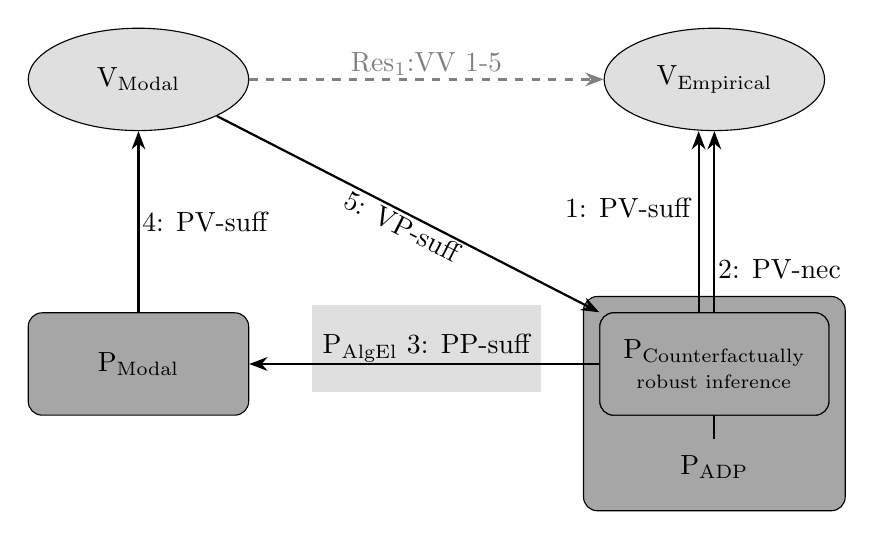
\begin{tikzpicture}[
  % Node Styles
  vnode/.style={ellipse, draw, fill=lightgray!50, text=black, minimum height=1.3cm, minimum width=2.8cm, align=center},
  pnode/.style={rectangle, rounded corners=5pt, draw, fill=gray!70, text=black, minimum height=1.3cm, minimum width=2.8cm, align=center, inner xsep=0.3cm, inner ysep=0.2cm},
  pbignode/.style={rectangle, rounded corners=5pt, fill=gray!70, text=black, minimum height=.3cm, minimum width=2.8cm, align=center, inner xsep=0.3cm, inner ysep=0.2cm},
  graybox/.style={rectangle, fill=lightgray!50, inner sep=4pt, minimum width=1.4cm, minimum height=1.1cm, anchor=center, align=center, text centered},
  % Arrow Styles
  solidarrow/.style={-Stealth, thick},
  dashedarrow/.style={dashed, -Stealth, thick, gray},
  textarrow/.style={align=center, inner sep=1pt}
]
\tikzset{font=\linespread{0.8}\selectfont} % Adjust line spacing

% Nodes
\node[vnode] (VModal) at (0,0) {V\textsubscript{Modal}};
\node[vnode, right=4.5cm of VModal] (VEmpirical) {V\textsubscript{Empirical}};
\node[pnode, below=2.3cm of VEmpirical] (PCounter) {P\textsubscript{Counterfactually} \\ \textsubscript{robust inference}};
\node[pbignode, below=0.3cm of PCounter] (PADP) {P\textsubscript{ADP}}; % P_ADP as text node, positioned below PCounter
\node[pnode, below=2.3cm of VModal] (PModal) {P\textsubscript{Modal}};

% Gray Box and Label
\node[graybox] (graybox1) at ($(PCounter)!0.5!(PModal) + (0,0.2)$) {P\textsubscript{AlgEl} 3: PP-suff};

% Arrows
\draw[dashedarrow] (VModal) -- node[midway, above, textarrow] {Res\textsubscript{1}:VV 1-5} (VEmpirical);
\draw[solidarrow] (PModal.north) -- node[midway, right, textarrow] {4: PV-suff} (VModal.south);
\draw[solidarrow] ([xshift=-.2cm]PCounter.north) --node[midway, above, textarrow, xshift=-.9cm] {1: PV-suff} ([xshift=-.2cm]VEmpirical.south); % Perpendicular arrow for 1
\draw[solidarrow] (PADP.north) -- node[midway, right, textarrow, yshift=.2cm] {2: PV-nec} (VEmpirical.south); % Arrow for 2, connecting PADP to PCounter
\draw[solidarrow] (PCounter) -- node[midway, above, sloped, textarrow, xshift=0.1cm] {} (PModal.east); % Corrected arrow for 3 to PModal.east
\draw[solidarrow] (VModal.south east) -- node[midway, below, sloped, textarrow] {5: VP-suff} (PCounter.north west);

% Background for nested P_ADP (fits PCounter only)
\begin{scope}[on background layer]
    \node[pnode, fill=gray!70, draw, fit=(PCounter)  (PADP), inner xsep=0.2cm, inner ysep=0.2cm] (PCounterBackground) {};
\end{scope}
\node[pnode, below=2.3cm of VEmpirical] (PCounter) {P\textsubscript{Counterfactually} \\ \textsubscript{robust inference}}; % Redraw PCounter on top

\end{tikzpicture}
\end{document}
